% !TeX root = thesis.tex
%--------------------------------------------------------------------%
%
% Template TA LaTeX Teknik Informatika ITERA.
% Editor: Radhinka Bagaskara, Martin C.T. Manullang, iwawiwi
% Version 2022-0.1
%
% Berdasarkan "Templat LaTeX Tesis Informatika ITB" oleh Petra Barus & Peb Ruswono Aryan
% https://github.com/petrabarus/if-itb-latex
%--------------------------------------------------------------------%
%
% Berkas ini berisi struktur utama dokumen LaTeX yang akan dibuat.
%
%--------------------------------------------------------------------%

\documentclass[12pt, a4paper, onecolumn, oneside, final]{report}

%-------------------------------------------------------------------%
%
% Konfigurasi dokumen LaTeX untuk laporan tesis IF ITB
%
% @author Petra Novandi
%
%-------------------------------------------------------------------%
%
% Berkas asli berasal dari Steven Lolong
%
%-------------------------------------------------------------------%

% Ukuran kertas
\special{papersize=210mm,297mm}

% Setting margin
\usepackage[top=3cm,bottom=3cm,left=4cm,right=3cm]{geometry}

\usepackage{mathptmx}

% Judul bahasa Indonesia
\usepackage[bahasa]{babel}

% Format citation
\usepackage[backend=bibtex,citestyle=ieee]{biblatex}

\usepackage[utf8]{inputenc}
\usepackage{graphicx}
\usepackage{titling}
\usepackage{blindtext}
\usepackage{sectsty}
\usepackage{chngcntr}
\usepackage{etoolbox}
\usepackage[bookmarks]{hyperref}
\hypersetup{
    colorlinks,
    citecolor=black,
    filecolor=black,
    linkcolor=black,
    urlcolor=black
}% Package untuk link di daftar isi.
\usepackage{titlesec}       % Package Format judul
\usepackage{parskip}
\usepackage{ragged2e}		% Alignment
\usepackage{multirow}		% Untuk bisa merge cell di tabel
\usepackage{tikz}			% Untuk menggambar kotak pas foto
\usepackage{setspace}		% Spacing paragraph
\usepackage{fancyhdr}		% Agar nomor halaman di pojok kanan atas
\usepackage{caption} 		% Caption gambar & tabel

% Setting supaya nomor halaman pertama dengan "chapter"
% berada di kanan atas
\fancypagestyle{plain}{%
	\fancyhf{}%
	\renewcommand{\headrulewidth}{0pt}
	\fancyhead[R]{\thepage}
}

% Line satu setengah spasi
\renewcommand{\baselinestretch}{1.5}

% Setting judul
\chapterfont{\centering \large}
\titleformat{\chapter}[display]%
  	{\large\centering\bfseries}%
  	{\chaptertitlename\ \thechapter}{0pt}%
  	{\large\bfseries\uppercase}
\titleformat{\section}%
	{\normalfont\normalsize\bfseries}{\thesection}{1em}{}
\titleformat{\subsection}%
	{\normalfont\normalsize\bfseries}{\thesubsection}{1em}{}
    
% Setting spacing di setiap judul chapter
\titlespacing*{\chapter}{0pt}{-30pt}{20pt}

% Setting nomor pada subbsubsubbab
\setcounter{secnumdepth}{4}

\makeatletter
% Command untuk variabel NIM
\newcommand{\nim}[1]{\def\@nim{120450081}}
\newcommand{\printnim}{\@nim}

% Command untuk variabel Dosen Pembimbing I & II
\newcommand{\namadosbinga}[1]{\def\@namadosbinga{#1}}
\newcommand{\namadosbingb}[1]{\def\@namadosbingb{#1}}
\newcommand{\nipdosbinga}[1]{\def\@nipdosbinga{#1}}
\newcommand{\nipdosbingb}[1]{\def\@nipdosbingb{#1}}
\newcommand{\printnamadosbinga}{\@namadosbinga}
\newcommand{\printnamadosbingb}{\@namadosbingb}
\newcommand{\printnipdosbinga}{\@nipdosbinga}
\newcommand{\printnipdosbingb}{\@nipdosbingb}
\newcommand{\dosbingA}[2]{\namadosbinga{#1} \nipdosbinga{#2}}
\newcommand{\dosbingB}[2]{\namadosbingb{#1} \nipdosbingb{#2}}

\makeatother

% Counter untuk figure dan table.
\counterwithin{figure}{chapter}
\counterwithin{table}{chapter}

% Supaya tidak ada garis di header
\renewcommand{\headrulewidth}{0pt}

% Setting penomoran caption gambar
\renewcommand{\thefigure}{\arabic{chapter}.\arabic{figure}}

% Setting penomoran caption tabel
\renewcommand{\thetable}{\arabic{chapter}.\arabic{table}}

% Mengkapitalkan judul Daftar Isi, Gambar, & Tabel
\addto\captionsbahasa{%
	\renewcommand{\contentsname}{DAFTAR ISI}%
	\renewcommand{\listfigurename}{DAFTAR GAMBAR}%
	\renewcommand{\listtablename}{DAFTAR TABEL}%
}

% english title
\providecommand\titleEN[1]{\providecommand\thetitleEN{#1}}

% Saya lupa ini buat apa (Radhinka)
%\renewcommand{\theHsection}{\thepart.section.\thesection}



\makeatletter

\makeatother

\bibliography{references}

\begin{document}
    \sloppy % mencegah text overflow.
    %Basic configuration
\title{Evaluasi Performa Hadoop dan Spark pada DigitalOcean menggunakan Hibench Benchmarking dalam Konfigurasi Pseudo Distributed} 	% Judul Tugas Akhir
\titleEN{Thesis Title}                  % Thesis Title
\author{Dimas Wahyu Saputro}		% Nama Mahasiswa
\nim{120450081}				% NIM Mahasiswa
\dosbingA%
    {Nama dan Gelar Pembimbing I}%	% Nama Dosen Pembimbing 1
    {NIP. 123456789}				% NIP Dosen Pembimbing 1
\dosbingB%
    {Tirta Setiawan, S.Pd., M.Si.}%	% Nama Dosen Pembimbing 2
    {NIP. 199008222022031003}				% NIP Dosen Pembimbing 2

\pagenumbering{roman}
\setcounter{page}{0}

\clearpage
\pagestyle{empty}

\begin{center}
\smallskip

    \begin{figure}[h]
    	\centering
    	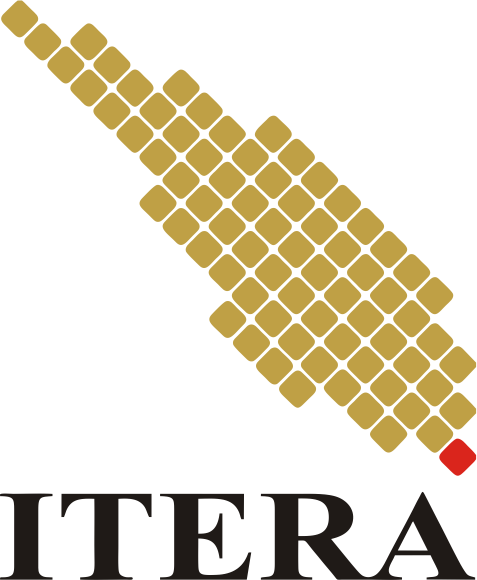
\includegraphics[width=2.1cm, height=2.5cm, keepaspectratio]{figures/itera-logo}
    \end{figure}

	\large \bfseries \MakeUppercase{\thetitle}
	\vfill

    \large \uppercase{TUGAS AKHIR}
    \vfill

    \normalsize \normalfont \theauthor\\
    \printnim
    \vfill

    \normalsize \bfseries
    \uppercase{
        Program Studi Sains Data \\
        Fakultas Sains\\
        Institut Teknologi Sumatera\\
        Lampung Selatan
    }\medskip

    %\thedate
    % automatic year
    \the\year{}

\end{center}

\clearpage
 % Hardcover
%\clearpage
\pagestyle{empty}
\phantomsection% 
\addcontentsline{toc}{chapter}{Halaman Judul}

\begin{center}
\smallskip

    \begin{figure}[h]
    	\centering
    	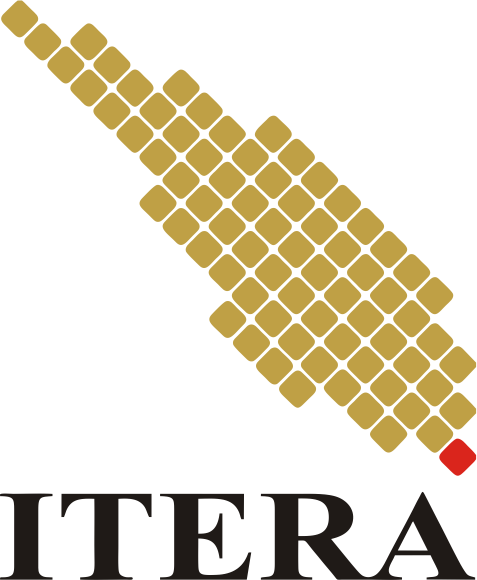
\includegraphics[width=2.1cm, height=2.5cm, keepaspectratio]{figures/itera-logo}
    \end{figure}

	\large \bfseries \MakeUppercase{\thetitle}
	\vfill

    \large \uppercase{Tugas Akhir}\\
    {\normalsize \normalfont Diajukan sebagai syarat untuk memperoleh gelar sarjana}
    \vfill

    \normalsize \normalfont \theauthor\\
    \printnim
    \vfill

    \normalsize \bfseries
    \uppercase{
        Program Studi Sains Data \\
        Fakultas Sains\\
        Institut Teknologi Sumatera\\
        Lampung Selatan
    }\medskip

    %\thedate
    % automatic year
    \the\year{}

\end{center}

\clearpage
 % Softcover
%\clearpage
\pagestyle{fancy}
\fancyhf{}
\fancyhead[R]{\thepage}
\phantomsection% 
\addcontentsline{toc}{chapter}{LEMBAR PENGESAHAN}

\begin{center}

%	\chapter*{\normalsize{Lembar Pengesahan}}
	\large \bfseries \MakeUppercase{Lembar Pengesahan} \linebreak
    
    \normalsize \normalfont \onehalfspacing \justify{
    Tugas Akhir Sarjana dengan judul \textbf{\thetitle} \ adalah benar dibuat oleh saya sendiri dan belum pernah dibuat dan diserahkan sebelumnya, baik sebagian ataupun seluruhnya, baik oleh saya ataupun orang lain, baik di Institut Teknologi Sumatera maupun di institusi pendidikan lainnya.}

	Lampung Selatan, \today{} % TODO: automatic date

	\setlength{\tabcolsep}{0pt}
%	\begin{tabular}{l@{\hskip 0.5in}r}
	\begin{tabular}{p{0.7\textwidth}p{0.3\textwidth}}
		Penulis, & \multirow{6}{*}{
			% Kotak pasfoto 3x4
			\begin{tikzpicture}
				\draw rectangle (3cm,4cm) node[pos=.5]{
					{\begin{tabular}{l}
					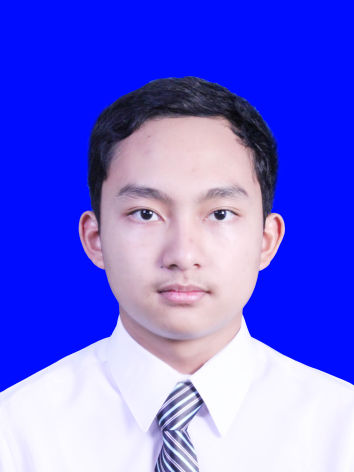
\includegraphics[width=.23\textwidth]{figures/pasfoto.jpg}
					\end{tabular}}};
			\end{tikzpicture}
			}\\
		& \\
		& \\
		& \\
		& \\
		\theauthor\\
		NIM \printnim
	\end{tabular}
	\vfill

	\centering Diperiksa dan disetujui oleh,
	\vspace{2em} % add space
	\justify
    \setlength{\tabcolsep}{0pt}
    \begin{tabular}{p{0.5\textwidth}p{0.5\textwidth}}
        \multicolumn{1}{c}{Pembimbing I,} & \multicolumn{1}{c}{Pembimbing II,} \\
        & \\
        & \\
        & \\
        & \\
		\multicolumn{1}{c}{\underline{\printnamadosbinga}} & \multicolumn{1}{c}{\underline{\printnamadosbingb}} \\
		\multicolumn{1}{c}{\printnipdosbinga} & \multicolumn{1}{c}{\printnipdosbingb} \\
    \end{tabular}
	\vfill

	\centering 
	\begin{tabular}{c}
		Disahkan oleh,\\
		Koordinator Program Studi Sains Data\\
		Fakultas Sains\\
		Institut Teknologi Sumatera
		\\
		\\
		\\
		\\
		\\
		\underline{Tirta Setiawan, S.Pd., M.Si.} \\ % TODO: make automatic
		NIP 199008222022031003 \\
	\end{tabular}
	
\end{center}
\clearpage

%\clearpage
\phantomsection% 
\addcontentsline{toc}{chapter}{Halaman Pernyataan Orisinalitas}

\begin{center}
	\smallskip
	
%	\chapter*{\normalsize{Halaman Pernyataan Orisinalitas}}
	\normalsize \bfseries \MakeUppercase{Halaman Pernyataan Orisinalitas} \linebreak
	
	\normalsize \onehalfspacing{
		Tugas Akhir ini adalah karya saya sendiri, dan semua sumber baik yang dikutip maupun dirujuk telah saya nyatakan benar}
	\vspace{3cm}
	
	\centering 
	\begin{tabular}{l l}
		Nama 			& : \theauthor \\
		& \\
		NIM 			& : \printnim \\
		& \\
		Tanda Tangan 	& : ................................... \\
		& \\
		Tanggal 		& : ................................... \\
	\end{tabular}
	
\end{center}
\clearpage

%\clearpage
\phantomsection% 
\addcontentsline{toc}{chapter}{Halaman Persetujuan Publikasi}

\begin{center}
	\smallskip
	
	\normalsize \bfseries \MakeUppercase{
		HALAMAN PERNYATAAN PERSETUJUAN PUBLIKASI \\
		TUGAS AKHIR UNTUK KEPENTINGAN AKADEMIS
	}\linebreak
	
	\normalsize \normalfont \onehalfspacing \justifying{
		Sebagai civitas akademik Institut Teknologi Sumatera, saya yang bertanda tangan di bawah ini:}
	
	\flushleft
	\setlength{\tabcolsep}{0pt}
	\begin{tabular}{l l}
		Nama 			&  : \theauthor\\
		NIM 			&  : \printnim\\
		Program Studi \	&  : Sains Data\\
		Jurusan 		&  : Fakultas Sains\\
		Jenis Karya 	&  : Tugas Akhir\\
	\end{tabular}

	\justifying
	demi pengembangan ilmu pengetahuan, menyetujui untuk memberikan kepada Institut Teknologi Sumatera \textbf{Hak Bebas Royalti Noneksklusif (Non-exclusive Royalty Free Right)} atas karya ilmiah saya yang berjudul: 
	
	\centering
	\textbf{\thetitle}
	
	\justifying
	beserta perangkat yang ada (jika diperlukan). Dengan Hak Bebas Royalti Noneksklusif ini Institut Teknologi Sumatera berhak menyimpan, mengalihmedia/formatkan, mengelola dalam bentuk pangkalan data (database), merawat, dan memublikasikan tugas akhir saya selama tetap mencantumkan nama saya sebagai penulis/pencipta dan sebagai pemilik Hak Cipta.
	
	Demikian pernyataan ini saya buat dengan sebenarnya. \\
	
	\centering
	Dibuat di : Lampung Selatan\\
	Pada tanggal : \today{}\\ % Automatic date
	\vspace{3cm}
	Yang menyatakan (\theauthor)
	
	
\end{center}
\clearpage

%
%\clearpage

\singlespacing{
	\textbf{\thetitle}\\
	\mbox{\theauthor \ (\printnim)}\\
	Pembimbing I \printnamadosbinga\\
	Pembimbing II \printnamadosbingb\\
}

%\chapter*{ABSTRAK}
\normalsize \bfseries \centering \MakeUppercase{Abstrak}
\phantomsection% 
\addcontentsline{toc}{chapter}{Abstrak}
\\[2\baselineskip]

%taruh abstrak bahasa indonesia di sini
\justifying \normalfont \normalsize{

}

\textbf{Kata Kunci}: Kata Kunci 1, Kata Kunci 2
\clearpage
%\clearpage

\begin{minipage}{\textwidth}
	\singlespacing{
	\textbf{\thetitleEN}\\
	\mbox{\theauthor \ (\printnim)}\\
	Pembimbing I \printnamadosbinga\\
	Pembimbing II \printnamadosbingb\\
}
\end{minipage}

%\chapter*{ABSTRAK}
\normalsize \bfseries \centering \MakeUppercase{Abstract}
\phantomsection% 
\addcontentsline{toc}{chapter}{Abstract}
\\[2\baselineskip]

%taruh abstrak bahasa inggris di sini
\justifying \normalfont \normalsize{

}

\textbf{Keyword}: Keyword 1, Keyword 2
\clearpage
%\clearpage

\normalsize \bfseries \centering \MakeUppercase{Motto}
\phantomsection% 
\addcontentsline{toc}{chapter}{Motto}
\\[2\baselineskip]

\justifying \normalfont{
	% Motto

}

\clearpage
%\clearpage

% PS: Ada bug dimana jika menge-build dari file ini, ada error. Tapi halamannya
% sendiri tidak error jika dibuild dari file lain. (Radhinka)

\normalsize \bfseries \centering \MakeUppercase{Persembahan}
\phantomsection% 
\addcontentsline{toc}{chapter}{Persembahan}
\\[2\baselineskip]

\justifying \normalfont{
	% Kata-kata persembahan
	\blindtext
}

\clearpage
%\clearpage

\normalsize \bfseries \centering \MakeUppercase{Kata Pengantar}
\phantomsection% 
\addcontentsline{toc}{chapter}{Kata Pengantar}
\thispagestyle{fancy}
\fancyhf{}
\fancyhead[R]{\thepage}
\\[2\baselineskip]

\normalsize \normalfont \justifying
(Tuliskan maksud penulisan laporan, misal “Laporan penelitian ini dimaksud kan untuk memenuhi salah ”.........Pada halaman ini mahasiswa berkesempatan untuk menyatakan terima kasih secara tertulis kepada pembimbing dan pihak lain yang telah memberi bimbingan, nasihat, saran dan kritik, kepada mereka yang telah membantu melakukan penelitian, kepada perorangan atau lembaga yang telah memberi bantuan keuangan, materi dan/atau sarana.

Cara menulis kata pengantar beraneka ragam, tetapi hendaknya menggunakan kalimat yang baku. Ucapan terima kasih agar dibuat tidak berlebihan dan dibatasi pada pihak yang terkait secara ilmiah (berhubungan dengan subjek/materi penelitian). 

\flushright{
	Tempat penyusunan TA, tgl-bln-thn\\
	Penulis,
	\\[5\baselineskip]
	\theauthor
}

\clearpage

%
%\tableofcontents
%\listoffigures
%\listoftables
%\clearpage

\chapter*{Daftar Simbol}
\thispagestyle{fancy}
\fancyhf{}
\fancyhead[R]{\thepage}

\justifying
(Tuliskan maksud penulisan laporan, misal “Laporan penelitian ini dimaksud kan untuk memenuhi salah ”.........Pada halaman ini mahasiswa berkesempatan untuk menyatakan terima kasih secara tertulis kepada pembimbing dan pihak lain yang telah memberi bimbingan, nasihat, saran dan kritik, kepada mereka yang telah membantu melakukan penelitian, kepada perorangan atau lembaga yang telah memberi bantuan keuangan, materi dan/atau sarana.

Cara menulis kata pengantar beraneka ragam, tetapi hendaknya menggunakan kalimat yang baku. Ucapan terima kasih agar dibuat tidak berlebihan dan dibatasi pada pihak yang terkait secara ilmiah (berhubungan dengan subjek/materi penelitian). 

    %----------------------------------------------------------------%
    % Konfigurasi Bab
    %----------------------------------------------------------------%
    \renewcommand{\chaptername}{BAB}
    % Bab: Arabic
    \renewcommand{\thechapter}{\Roman{chapter}}
    % Sub-bab: Roman
    \renewcommand\thesection{\arabic{chapter}.\arabic{section}}
    
    % Setting supaya nomor halaman pertama dengan "chapter"
    % berada di tengah bawah
    \fancypagestyle{plain}{%
    	\fancyhf{}%
    	\renewcommand{\headrulewidth}{0pt}
    	\fancyhead[]{}
    	\fancyfoot[C]{\thepage}
    }
    %----------------------------------------------------------------%

    %----------------------------------------------------------------%
    % Daftar Bab
    % Untuk menambahkan daftar bab, buat berkas bab misalnya `chapter-6` di direktori `chapters`, dan masukkan ke sini.
    %----------------------------------------------------------------%

    % Reset penomoran halaman menjadi 1
    \clearpage
    \setcounter{page}{1}
    \pagenumbering{arabic}

    \justifying
    \chapter{Pendahuluan}

\pagestyle{plain}

\section{Latar Belakang}

Pengolahan dan analisis data telah menjadi bagian penting dalam berbagai aspek kehidupan modern \cite{vermaBigDataManagement2016}. Organisasi, perusahaan, dan lembaga pemerintah mengandalkan data untuk pengambilan keputusan, inovasi produk, pengembangan layanan pelanggan, dan banyak aspek lainnya. Seiring dengan meningkatnya volume data yang dihasilkan setiap hari, tantangan utama yang dihadapi adalah bagaimana mengelola dan menganalisis data ini dengan efisien dan cepat \cite{ahmadvandGapproxUsingGallup2019}. Beberapa solusi telah tersedia untuk mengatasi masalah ini. Salah satu solusi yang paling efisien adalah komputasi terdistribusi. 

Komputasi terdistribusi adalah cara untuk mencapai paralelisme dengan menggabungkan beberapa mesin independen yang berbeda \cite{bhattacharyaEvaluatingDistributedComputing2021}. Dalam komputasi terdistribusi, data besar dibagi ke dalam sejumlah \textit{node} atau server yang bekerja bersama-sama untuk mengolahnya. Dua teknologi yang umum digunakan dalam komputasi terdistribusi ini adalah Apache Hadoop dan Apache Spark. Hadoop dan Spark adalah dua platform komputasi \textit{big data} yang paling populer dan banyak digunakan di seluruh dunia. \textit{Platform} ini menawarkan berbagai kemampuan untuk mengelola, menyimpan, dan menganalisis data dalam skala besar. 

MapReduce adalah alat yang digunakan untuk komputasi terdistribusi, dirancang khusus untuk menulis, membaca, dan memproses jumlah data yang besar \cite{deanMapReduceSimplifiedData2004}. Pemrosesan data dalam MapReduce ini terdiri dari tiga tahap: fase \textit{Map}, fase \textit{Shuffle}, dan fase \textit{Reduce}. Dalam teknik ini, berkas-berkas besar dibagi menjadi beberapa blok kecil dengan ukuran yang sama dan didistribusikan ke seluruh klaster untuk penyimpanan. MapReduce dan sistem file terdistribusi (HDFS) adalah bagian inti dari sistem Hadoop, sehingga komputasi dan penyimpanan bekerja bersama-sama di seluruh \textit{node} yang membentuk klaster komputer \cite{samadiComparativeStudyHadoop2016}. Hadoop MapReduce memerlukan akses ke penyimpanan untuk membaca dan menulis data, sehingga dapat memperlambat proses komputasi, sehingga hadirlah Spark.

Spark, di sisi lain, menawarkan teknologi \textit{Resilient Distributed Datasets} (RDDs) untuk mendukung proses \textit{Map} dan \textit{Reducing} secara lebih efektif dan cepat \cite{ahmadvandGapproxUsingGallup2019}. Spark bukan hanya alternatif Hadoop, tetapi juga menyediakan berbagai fungsi, misalnya mendukung \textit{MLib}, \textit{GraphX}, dan \textit{Spark streaming} untuk analisis data besar \cite{zahariaSparkClusterComputing2010}. Spark menggunakan memori untuk menyimpan data sehingga dapat mengurangi siklus baca dan tulis. Perbedaan mendasar ini mengakibatkan menarik untuk melihat perbandingan performa antara keduanya. Salah satu cara untuk membandingkan performa keduanya adalah menggunakan tolok ukur Hibench.

Tolok ukur HiBench adalah salah satu tolok ukur kinerja yang paling sering digunakan. HiBench mencakup sejumlah tugas \textit{benchmarking} yang mencerminkan berbagai jenis pemrosesan data, seperti pengolahan batch, aliran data, \textit{query}, atau pun \textit{machine learning} \cite{huangHiBenchBenchmarkSuitea}. Oleh karena itu, HiBench adalah alat yang cocok untuk mengukur dan membandingkan kinerja antara Hadoop dan Spark dalam berbagai skenario penggunaan.

Penelitian tentang evaluasi performa Hadoop dan Spark menggunakan HiBench telah beberapa kali dilakukan. Shi et al. \cite{shiClashTitansMapReduce2015} melakukan penelitian dengan dua alat yang dirancang untuk mengukur kinerja MapReduce dan Spark dalam berbagai skenario beban kerja. Penelitian ini mengevaluasi kinerja dalam pekerjaan \textit{batch} dan iteratif, dengan fokus pada komponen-komponen penting seperti \textit{shuffle}, dan \textit{caching}. Hasil penelitian mereka menunjukkan bahwa Spark lebih cepat daripada Hadoop dalam beberapa kasus, terutama ketika menangani tugas-tugas pemrosesan data yang lebih kecil. Namun, ketika ukuran data meningkat, Hadoop terbukti lebih efisien. Selanjutnya, perbandingan kinerja antara Hadoop dan Spark juga disorot oleh penelitian Samadi et al. \cite{samadiComparativeStudyHadoop2016}, yang menggunakan delapan tolok ukur dari HiBench. Penelitian ini menunjukkan bahwa Spark cenderung lebih efisien ketika menangani data dalam jumlah kecil atau saat memproses tugas dalam memori, sementara Hadoop lebih sukses ketika beban kerja melibatkan operasi I/O penyimpanan yang intensif. Selain itu, penelitian oleh Satish dan Rohan \cite{gopalaniComparingApacheSpark2015} menyoroti perbandingan kinerja antara Hadoop dan Spark khususnya dalam konteks algoritma \textit{K-means}. Penelitian itu menemukan bahwa Spark dapat mencapai kecepatan hingga tiga kali lipat dibandingkan Hadoop, dengan catatan bahwa performa Spark sangat bergantung pada ukuran memori yang memadai.

Berdasarkan penelitian sebelumnya, penelitian ini bertujuan untuk menyelidiki perbandingan kinerja antara Hadoop dan Spark dengan menggunakan tolok ukur HiBench dengan studi kasus tertentu. Dengan pemahaman mendalam mengenai kekuatan dan kelemahan masing-masing \textit{platform} dalam berbagai konteks pemrosesan data, organisasi atau peneliti dapat membuat keputusan yang lebih informasional saat memilih \textit{platform} yang paling sesuai dengan kebutuhan mereka. Selain itu, penelitian ini akan dilakukan dengan memanfaatkan Infrastruktur sebagai Layanan (IaaS) yang disediakan oleh \textit{DigitalOcean}, memungkinkan penggunaan sumber daya komputasi dalam skala yang fleksibel dan efisien. Dengan demikian, penelitian ini akan memberikan kontribusi berharga dalam membantu pemangku kepentingan dalam mengoptimalkan pemrosesan data dalam lingkungan komputasi terdistribusi.

\section{Rumusan Masalah}
Adapun rumusan masalah dalam penelitian ini adalah sebagai berikut:
\begin{enumerate}
	\item Bagaimana implementasi HiBench pada Hadoop dan Spark di DigitalOcean?
	\item Bagaimana kinerja Hadoop dan Spark ketika diuji menggunakan  beban kerja \textit{Micro Benchmarks} yang disediakan oleh HiBench?
	\item Bagaimana perbandingan kinerja antara Hadoop dan Spark dalam mode pseudo-distribusi dalam konteks pemrosesan data dalam skala besar dengan menggunakan tolok ukur HiBench?
\end{enumerate}

\section{Tujuan}
Penelitian ini memiliki tujuan, yaitu:
	\begin{enumerate}
		\item Untuk mengetahui implementasi HiBench pada Hadoop dan Spark di DigitalOcean
		\item Untuk mengukur kinerja Hadoop dan Spark ketika diuji menggunakan  beban kerja \textit{Micro Benchmarks} yang disediakan oleh HiBench
		\item Untuk membandingkan kinerja antara Hadoop dan Spark dalam mode pseudo-distribusi saat memproses data dalam skala besar dengan menggunakan tolok ukur HiBench
	\end{enumerate}

\section{Manfaat}
Hasil dari penelitian ini diharapkan akan memberikan manfaat sebagai berikut:
\begin{enumerate}
	\item 
	Penelitian ini akan memberikan informasi yang berguna bagi organisasi yang sedang mempertimbangkan pemilihan platform \textit{Big Data}, sehingga mereka dapat membuat keputusan yang lebih terinformasi.	
	\item
	Penelitian ini akan membantu dalam memahami lebih dalam kinerja Hadoop dan Spark dalam berbagai skenario pemrosesan data.
	\item
	Hasil dari penelitian ini dapat menjadi dasar untuk penelitian lebih lanjut dalam pengembangan dan peningkatan platform \textit{Big Data.}
\end{enumerate}

\section{Batasan Masalah}
Penelitian ini memiliki beberapa batasan yang perlu diperhatikan sebagai berikut:
	\begin{enumerate}
		\item 
		Penelitian ini akan fokus pada perbandingan kinerja antara Hadoop dan Spark dalam mode \textit{pseudo-distributed.}
		\item
		Pengujian kinerja akan menggunakan HiBench, sebuah tolok ukur kinerja yang umum digunakan dalam penelitian \textit{Big Data.}
		\item
		Implementasi Hadoop dalam lingkungan komputasi awan akan menggunakan salah satu penyedia awan, yaitu \textit{DigitalOcean}.
		\item
		Penelitian ini akan berfokus pada aspek kinerja. Aspek lain seperti keamanan dan administrasi tidak akan dibahas secara rinci.
	\end{enumerate}

%\section{Metodologi}
%
%Tuliskan semua tahapan yang akan dilalui selama pelaksanaan tugas akhir. Tahapan ini spesifik untuk menyelesaikan persoalan tugas akhir. Tahapan studi literatur tidak perlu dituliskan karena ini adalah pekerjaan yang harus Anda lakukan selama proses pelaksanaan tugas akhir.
%
%\section{Sistematika Pembahasan}
%
%Subbab ini berisi penjelasan ringkas isi per bab. Penjelasan ditulis satu paragraf per bab buku.

    \chapter{Tinjauan Pustaka}

\section{Studi Terkait}
\blindtext

\section{Dasar Teori}
Penelitian ini menggunakan beberapa teori dasar pendukung agar dapat memperjelas proses penelitian dan memberikan pemahaman lebih lanjut. Teori-teori dasar yang berhubungan dan digunakan dalam penelitian ini adalah sebagai berikut.
\subsection{MapReduce}
MapReduce adalah model pemrograman dan implementasi teknik pemrosesan data berukuran besar yang pertama kali dipopulerkan oleh Google pada tahun 2004\cite{kaliaAnalysisHadoopMapReduce2021}. MapReduce menawarkan pemrosesan data yang dapat diandalkan serta \textit{fault-tolerant manner} (tahan terhadap kesalahan).  MapReduce berjalan secara paralel dan berada pada lingkungan komputasi terdistribusi \cite{cTaskFailureResilience2020}. Model ini mengadopsi arsitektur tersentraliasi, yaitu satu \textit{node} berperan sebagai \textit{master} dan \textit{node} yang lain berperan sebagai \textit{workers} atau \textit{slave} \cite{herodotouHadoopPerformanceModels2011, bakratsasHadoopMapReducePerformance2018}. \textit{Master node} bertanggung jawab untuk melakukan penjadwalan kerja, dan \textit{slave node} berperan untuk menjalankan eksekusi kerja. 

\begin{figure}[h!]
    \centering
    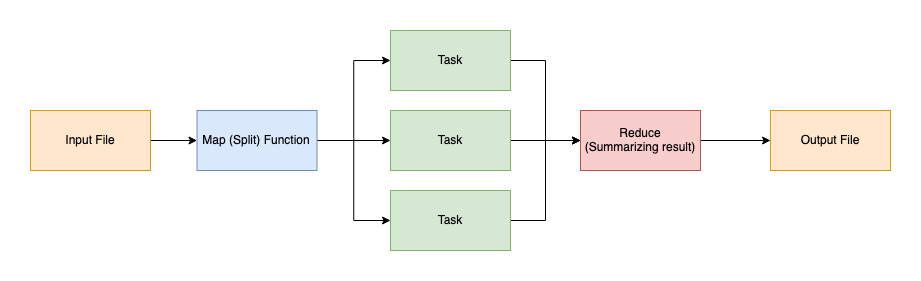
\includegraphics[width=1\textwidth]{figures/ch02/mapreduce-scheme.png}
    \caption{Cara Kerja MapReduce}
    \label{fig:mapreduce-flow}
\end{figure}

MapReduce terdiri dari fungsi \textit{Map} dan fungsi \textit{Reduce} \cite{gandomiHybSMRPHybridScheduling2019}. Kedua fungsi ini tersebar di seluruh \textit{slave node} yang terhubung dalam klaster dan berjalan secara paralel. Fungsi \textit{Map} berperan untuk membagi masalah besar menjadi masalah yang lebih kecil dan mendistribusikannya ke \textit{slave node}. Hasil pemrosesan dari \textit{slave node} akan dikumpulkan oleh \textit{master node} melalui fungsi \textit{Reduce}. Sesuai dengan Gambar \ref{fig:mapreduce-flow}, hasil dari proses \textit{Reduce} yang akan dikirimkan sebagai hasil akhir proses MapReduce.  

Implementasi MapReduce pada \textit{Word Count}\cite{KOMPARASIKECEPATANHADOOP} dapat dilihat pada Gambar \ref{fig:mapreduce-wordcount}. Pada proses MapReduce, data masukan akan melalui beberapa tahapan pemrosesan. Pertama, data akan dipecah menjadi bagian-bagian yang lebih kecil pada proses pemecahan data masukan (\textit{splitting}). Dalam kasus Hadoop MapReduce, data idealnya akan dipecah menjadi beberapa blok berukuran maksimal 128MB.

\begin{figure}[h!]
    \centering
    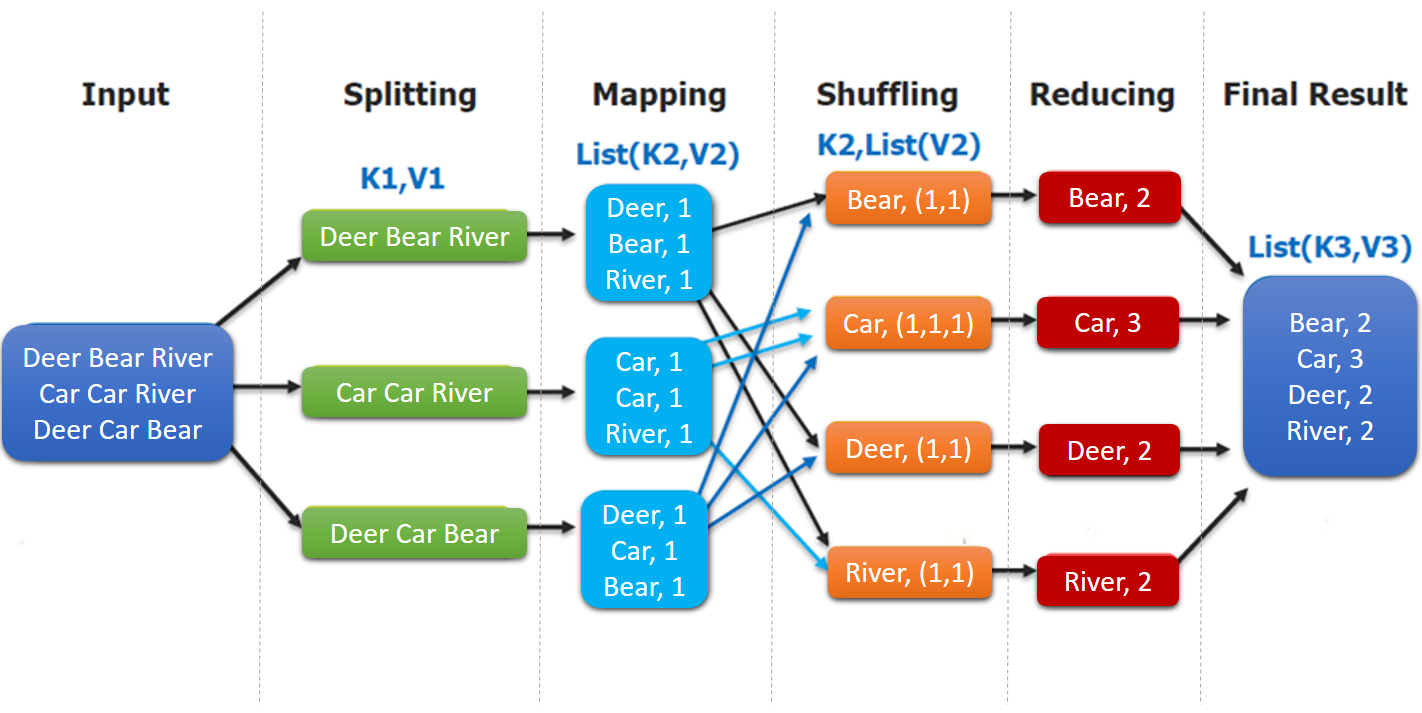
\includegraphics[width=0.9\textwidth]{figures/ch02/map-reduce-word-count-oreilly.png}
    \caption{Implementasi MapReduce pada Word Count. Sumber:  \cite{MapReduceDistributedComputing}}
    \label{fig:mapreduce-wordcount}
\end{figure}

Kemudian, blok data tersebut akan diproses lebih lanjut pada tahap pemetaan (\textit{mapping}). Pemetaan merupakan salah satu tahapan terpenting dalam MapReduce. Pada tahap ini, blok data yang sudah dipecah akan diproses untuk menghasilkan pasangan kunci-nilai (\textit{key-value pairs}) sementara, seperti pada contoh kasus \textit{wordcount} yang menghasilkan pasangan kunci-nilai \textit{Dear:1, Bear:1, dan River:1}. Pemetaan dapat melibatkan satu atau beberapa mesin pekerja (\textit{worker}) yang memproses blok data secara paralel.

Selanjutnya adalah tahap pengocokan (\textit{shuffling}) di mana pasangan kunci-nilai hasil pemetaan yang tersebar di beberapa mesin akan dikumpulkan berdasarkan kesamaan kuncinya agar bisa diproses lebih lanjut. Misalnya semua pasangan dengan kunci \textit{Bear} dikumpulkan dalam satu mesin.

Pada tahap terakhir yaitu pengurangan (\textit{reducing}), dilakukan agregasi terhadap pasangan kunci-nilai dengan kunci yang sama untuk menghasilkan keluaran akhir. Seperti pada contoh kasus \textit{wordcount}, pasangan \textit{Bear:1} dan \textit{Bear:1} akan dijumlahkan menjadi \textit{Bear:2} oleh proses pengurangan.

\subsection{Apache Hadoop}
Apache Hadoop adalah perangkat lunak sumber terbuka yang ditulis dengan bahasa pemrograman Java untuk pemrosesan dan penyimpanan data menggunakan komputasi terdistribusi (\cite{ApacheHadoop}). Hadoop dapat diinstalasi pada satu \textit{node} komputer, atau ratusan \textit{node} komputer yang digabungkan dalam sebuah klaster (\cite{maneasEvolutionHadoopDistributed2018}). Berkaitan dengan pemrosesan data, Hadoop mengimplementasikan model MapReduce untuk pemrosesan data secara paralel dan cepat. Selain itu, Hadoop menyediakan sistem penyimpanan data terdistribusi yang dikenal sebagai Hadoop Distributed File System (HDFS) untuk akses data, pemrosesan, dan komputasi \cite{dabasAnalysisCommentsYoutube2019}. Arsitektur Hadoop secara umum dapat dilihat pada Gambar \ref{fig:hadoop-str}.

\begin{figure}[h!]
    \centering
    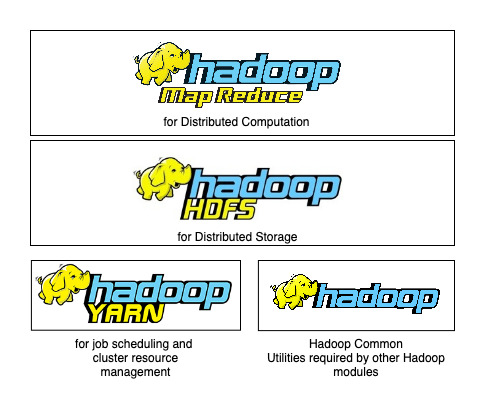
\includegraphics[width=0.9\textwidth]{figures/ch02/hadoop-str}
    \caption{Arsitektur Hadoop}
    \label{fig:hadoop-str}
\end{figure}



\subsubsection{Cara Kerja Apache Hadoop}
\blindtext
\subsubsection{Hadoop Distributed File System (HDFS)}
\blindtext
\subsubsection{Hadoop Map Reduce}
\blindtext
\subsection{Apache Spark}
\blindtext
\subsection{HiBench Suite}
\blindtext
\subsubsection{Jenis-jenis Beban Kerja pada HiBench}
    \chapter{METODOLOGI PENELITIAN}
\section{Tempat dan Jadwal Kegiatan Penelitian}
Dalam melaksanakan sebuah penelitian, perencanaan waktu merupakan komponen kritis yang memastikan alur penelitian dapat berjalan dengan terstruktur dan sistematis. Gambar \ref{fig:jadwal-penelitian} menyajikan jadwal penelitian yang telah dirancang untuk penelitian ini. Jadwal tersebut mencakup rentang waktu mulai dari September 2023 hingga April 2024 dan menguraikan berbagai kegiatan yang akan dilakukan selama periode tersebut. Selanjutnya, penelitian ini akan dilaksanakan di Laboratorium Komputer, Institut Teknologi Sumatera.

\begin{figure}[h!]
    \centering
    \includegraphics[width=1\textwidth]{figures/ch03/Timeline-2.png}
    \caption{Jadwal Penelitian}
    \label{fig:jadwal-penelitian}
\end{figure}


\section{Alur Penelitian}
Adapun diagram alir penelitian ini ditunjukkan pada Gambar \ref{fig:diagram alir} terdapat enam tahapan. Langkah awal yang dilakukan pada penelitian ini adalah melakukan identifikasi masalah, yaitu proses mencari, menghimpun, serta menemukan permasalahan yang nantinya akan diselesaikan. Setelah melakukan identifikasi masalah, langkah selanjutnya adalah studi literatur. Studi literatur adalah tahapan untuk mencari solusi dari permasalahan yang sebelumnya sudah kita definisikan. Pencarian solusi ini dapat melalui membaca referensi ilmiah terdahulu, baik melalui jurnal, buku, dokumentasi resmi, tesis, dan lain-lain. Tahapan ini akan memberikan pemahaman mendasar mengenai permasalahan yang sudah didapatkan sebelumnya. 

\begin{figure}[h!]
    \centering
    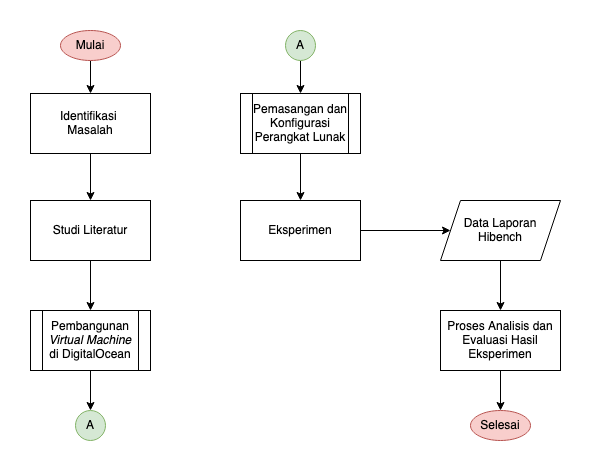
\includegraphics[width=0.9\textwidth]{figures/ch03/Diagram Tugas Akhir.png}
    \caption{Diagram Alir Penelitian}
    \label{fig:diagram alir}
\end{figure}

Kemudian, penelitian ini akan dilanjutkan pada tahap membangun \textit{virtual machine} di DigitalOcean. DigitalOcean adalah perusahaan penyedia layanan awan \textit{Infrastructure as a Service} (IaaS) yang memberikan banyak pilihan kepada pengguna untuk menggunakan berbagai jenis layanan sesuai dengan kebutuhan, salah satunya yaitu \textit{virtual machine}. \textit{Virtual Machine} tersebut dapat dihentikan atau dihapus kapanpun saat tidak lagi diperlukan. Ketika infrastruktur sudah siap digunakan, penelitian dilanjutkan ke tahap pemasangan perangkat lunak, seperti Hadoop, Spark, dan HiBench. Selanjutnya dilakukan eksperimen pada beban kerja \textit{Micro Benchmarks}. Akhirnya, hasil dari eksperimen akan digunakan untuk proses analisis dan evaluasi.

\section{Penjabaran Langkah Penelitian}
Adapun untuk lebih memperjelas lagi dari setiap langkah yang ada pada Gambar \ref{fig:diagram alir}, dijabarkan secara rinci tahapan-tahapan yang dilakukan pada penelitian ini.

\subsection{Identifikasi Masalah dan Studi Literatur}
Langkah awal penelitian ini adalah identifikasi masalah dan studi literatur. Identifikasi masalah dapat dipahami sebagai tahapan mendefinisikan masalah sehingga masalah tersebut dapat terukur dan jelas untuk dijadikan landasan dalam latar belakang penelitian. Setelah masalah berhasil diidentifikasi, langkah selanjutnya adalah studi literatur yang mana dalam proses ini dilakukan pengumpulan berbagai macam informasi, referensi, dan konsep dasar yang menjadi landasan dasar dari penelitian. Langkah ini dapat dilakukan melalui membaca artikel ilmiah pendukung, buku-buku yang ditulis oleh para ahli, dan jika berkaitan dengan pemrograman dapat melihat dari dokumentasi resmi. Pada tahap ini juga dilakukan analisis terhadap penelitian terdahulu dan dibandingkan dengan identifikasi masalah yang didapatkan untuk membuka celah penelitian baru sehingga penelitian ini dapat bermanfaat. 

\subsection{Membangun \textit{Virtual Machine} di DigitalOcean}
Konfigurasi perangkat keras merupakan aspek penting dalam mengevaluasi kinerja aplikasi \textit{big data} berbasis Hadoop dan Spark. DigitalOcean, sebagai penyedia layanan infrastruktur sebagai layanan (IaaS), memberikan pengguna kebebasan penuh untuk membuat, mengonfigurasi, dan mengelola berbagai infrastruktur yang telah disediakan. Dalam konteks penelitian ini, diperlukan penggunaan mesin virtual, yang dalam DigitalOcean dikenal sebagai "Droplets," yang memungkinkan untuk menyesuaikan berbagai aspek seperti sistem operasi, kapasitas penyimpanan, jumlah prosesor, dan parameter lainnya sesuai dengan kebutuhan spesifik penelitian.

\begin{table}[h!]
	\centering
	\caption{Konfigurasi Perangkat Keras}
	\begin{tabular}{|ll|}
		\hline
		\multicolumn{1}{|c|}{\textbf{Nama Parameter}}    & \multicolumn{1}{c|}{\textbf{Nilai Parameter}} \\ \hline
		\multicolumn{1}{|l|}{\textbf{Lokasi Pusat Data}} & Singapore - Datacenter 1 - SGP1               \\ \hline
		\multicolumn{1}{|l|}{\textbf{Sistem Operasi}}    & Ubuntu 20.04 (LTS) x64                        \\ \hline
		\multicolumn{1}{|l|}{\textbf{Jenis Droplet}}     & Basic                                         \\ \hline
		\multicolumn{1}{|l|}{\textbf{Prosesor}}          & Premium AMD - 4 Core                          \\ \hline
		\multicolumn{1}{|l|}{\textbf{Memori}}            & 8 GB                                          \\ \hline
		\multicolumn{1}{|l|}{\textbf{Penyimpanan}}       & 160 GB NVMe SSD                               \\ \hline
	\end{tabular}
	\label{table:conf-hardware}
\end{table}

Penelitian ini mengadopsi mode \textit{pseudo-distributed} yang memungkinkan penggunaan hanya satu \textit{virtual machine} dalam konfigurasi \textit{single node}. Walaupun hanya menggunakan satu \textit{virtual machine}, mode \textit{pseudo-distributed} memungkinkan setiap proses dalam klaster beroperasi secara independen, menciptakan lingkungan di mana semua proses berjalan mandiri satu sama lain. Hal ini memungkinkan untuk lebih berfokus pada pengumpulan data dan analisis, tanpa perlu melakukan konfigurasi yang rumit terkait dengan pengaturan klaster. Spesifikasi perangkat keras yang digunakan untuk \textit{virtual machine} dalam mode \textit{pseudo-distributed} sesuai pada Tabel \ref{table:conf-hardware}. Penjelasan lengkap tentang pembuatan \textit{virtual machine} (VM) pada \textit{platform} DigitalOcean dan cara mengakses VM tersebut disajikan pada Lampiran \ref{appendix:A}.

\subsection{Pemasangan dan Konfigurasi Perangkat Lunak}
Pemasangan dan konfigurasi perangkat lunak merupakan hal yang krusial dalam penelitian ini. Perangkat lunak yang diperlukan ditunjukkan pada Tabel \ref{table:software-needs}.

\begin{table}[h]
	\centering
	\caption{Perangkat Lunak yang Dibutuhkan}
		\begin{tabular}{|c|p{9cm}|}
		\hline
			\textbf{Perangkat Lunak} & \multicolumn{1}{c|}{\textbf{Deskripsi}}                                                                                \\ \hline
			Ubuntu 20.04 LTS x64     & Sistem operasi Linux berbasis Ubuntu  \\ \hline
			Git                      & Sistem kontrol versi untuk mengelola perubahan dalam kode sumber perangkat lunak                                       \\ \hline
			Maven                    & Perangkat lunak manajemen proyek Java                            \\ \hline
			Java 8                   & \multirow{3}{*}{Bahasa pemrograman dasar}                                 \\ \cline{1-1}
			Python 3.7               &                                                                                                                        \\ \cline{1-1}
			Scala 2.x               &                                                                                                                        \\ \hline
			Hadoop                & Perangkat lunak pengolahan data terdistribusi untuk penyimpanan dan manajemen data besar                               \\ \hline
			Spark               & Kerangka kerja pemrosesan data terdistribusi yang berjalan di atas Hadoop                                              \\ \hline
			Hibench   & Alat yang digunakan untuk mengukur kinerja Hadoop dan Spark                                                            \\ \hline
		\end{tabular}
	\label{table:software-needs}
\end{table}

Alur kerja instalasi perangkat lunak dalam penelitian ini dapat dilihat pada Gambar \ref{fig:alurkerja-soft}. Pada gambar, terdapat tiga bagian utama, yaitu \textit{prerequisites} (perangkat lunak prasyarat) ditandai dengan warna biru, alat penyimpanan dan pemrosesan \textit{Big Data} ditandai dengan warna oren, dan alat untuk mengukur kinerja \textit{big data} ditandai dengan warna hijau. Semua perangkat lunak dijalankan pada sistem operasi Ubuntu 20.04 LTS x64.

\begin{figure}[h]
    \centering
    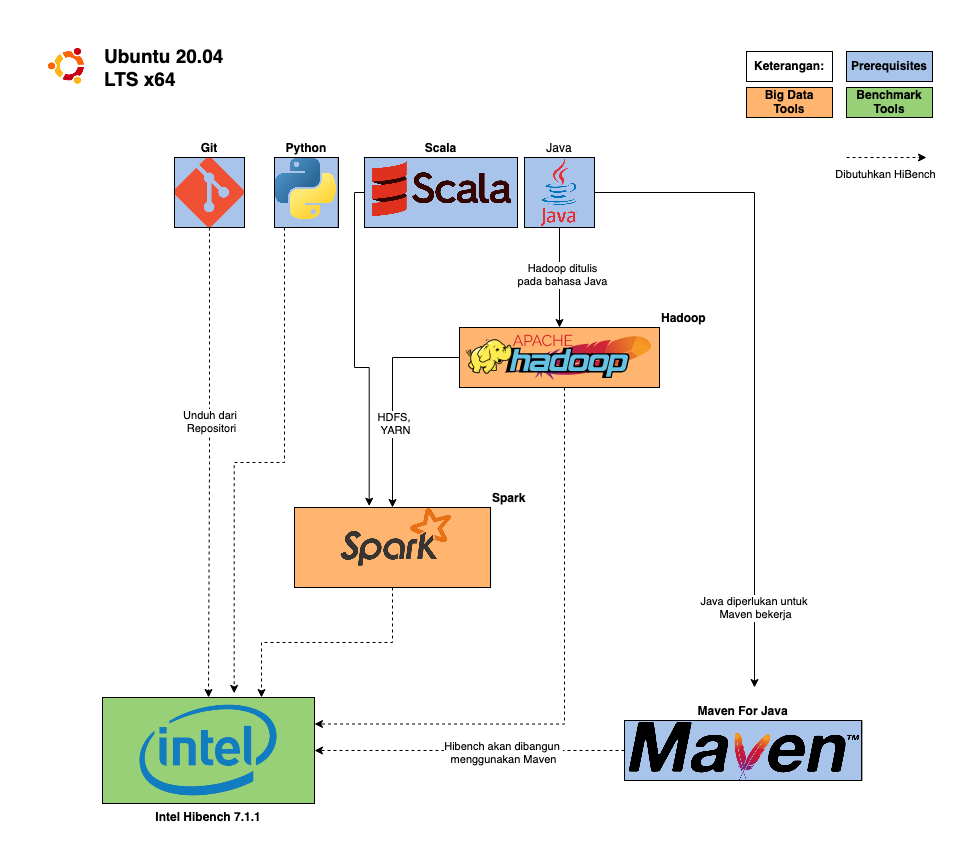
\includegraphics[width=1\textwidth]{figures/ch03/alurkerja-soft.png}
    \caption{Alur Instalasi Perangkat Lunak}
    \label{fig:alurkerja-soft}
\end{figure}

\subsubsection{Instalasi Perangkat Lunak Prasyarat}
Ada beberapa perangkat lunak yang perlu diimplementasikan sebelum memasang Hadoop, Spark, Hive, dan HiBench, yaitu:
\begin{enumerate}
	\item Ubuntu 20.04 LTS x64
	\item Git
	\item Java 8 dan Maven
	\item Python 3.7
	\item Scala 2.x
\end{enumerate}

Pemasangan dan konfigurasi perangkat lunak pada tahapan ini tidak membutuhkan urutan. Akan tetapi, pada penelitian ini dibuatkan alur untuk pemasangan dan konfigurasi perangkat lunak prasyarat seperti pada Gambar \ref{fig:prasyarat-flow}. Penjelasan lengkap mengenai tata cara instalasi dan konfigurasi perangkat lunak prasyarat ini disajikan pada Lampiran \ref{appendix:B}. 

\begin{figure}[h!]
    \centering
    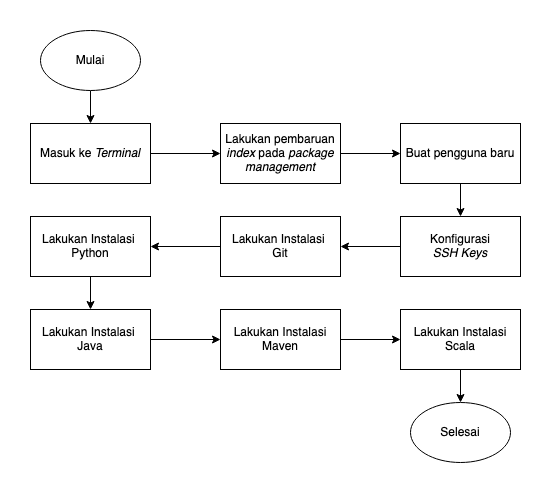
\includegraphics[width=0.75\textwidth]{figures/ch03/prasayarat-flow.png}
    \caption{Alur Instalasi Perangkat Lunak Prasyarat}
    \label{fig:prasyarat-flow}
\end{figure}


\subsubsection{Instalasi dan Konfigurasi Hadoop}
Hadoop adalah perangkat lunak \textit{open source} yang efektif dalam menyimpan dan memproses data dalam skala besar. Daripada menggunakan satu komputer besar untuk menyimpan dan memproses data, Hadoop memungkinkan pengklasteran beberapa komputer untuk menganalisis set data besar secara paralel dengan lebih cepat. Ada beberapa perangkat lunak prasyarat yang perlu dipasang sebelum menggunakan Hadoop. Setelah perangkat lunak prasyarat berhasil dipasang, Hadoop juga dapat dipasang mengikuti panduan lengkap pada Lampiran \ref{appendix:C}. 
Secara umum, alur yang harus dilakukan meliputi pengunduhan berkas Hadoop. Selanjutnya akan dilakukan pengubahan kepemilikan berkas ke \textit{user hdfsuser}. Karena Hadoop tidak mendukung IPv6, maka fitur ini perlu dimatikan juga. Alur pemasangan dan konfigurasi Hadoop lebih jelas sesuai dengan Gambar \ref{fig:hadoop-flow}.

\begin{figure}[h!]
    \centering
    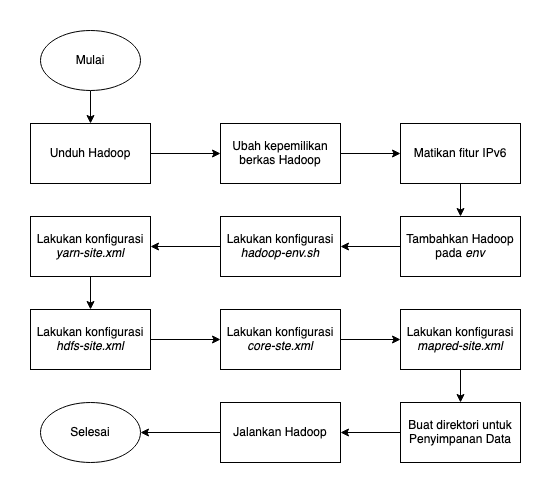
\includegraphics[width=0.6\textwidth]{figures/ch03/hadoop-flow.png}
    \caption{Alur Instalasi dan Konfigurasi Hadoop}
    \label{fig:hadoop-flow}
\end{figure}

\subsubsection{Instalasi dan Konfigurasi Spark}
Apache Spark adalah sebuah kerangka kerja pengolahan data terdistribusi yang sangat cepat dan efisien. Spark dan Hadoop memiliki hubungan yang erat. Spark dapat berjalan di atas \textit{Hadoop Distributed File System} (HDFS) dan dapat menggunakan Hadoop YARN sebagai manajer sumber daya. Oleh karena itu, instalasi Spark membutuhkan Hadoop sudah terpasang lebih dahulu. Alur pemasangan dan konfigurasi spark terlihat seperti pada Gambar \ref{fig:spark-flow}. Apabila Hadoop sudah berhasil terpasang, langkah selanjutnya adalah memasang Spark seperti pada Lampiran \ref{appendix:D}.

\begin{figure}[h]
    \centering
    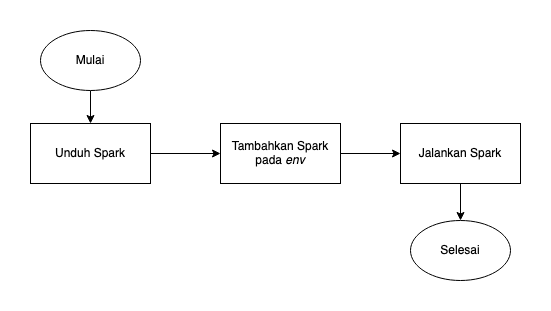
\includegraphics[width=0.7\textwidth]{figures/ch03/spark-flow.png}
    \caption{Alur Instalasi dan Konfigurasi Spark}
    \label{fig:spark-flow}
\end{figure}

\subsubsection{Instalasi dan Konfigurasi HiBench}
Sebelum melakukan eksperimen, diperlukan suatu perangkat lunak pengukuran kinerja sistem \textit{Big Data}, yaitu HiBench. HiBench tidak dapat digunakan secara langsung ketika sudah berhasil diunduh, melainkan harus dilakukan pembangunan beberapa modul yang dibutuhkan dengan Maven dan konfigurasi beberapa parameter. Secara umum, alur instalasi dan konfigurasi HiBench sesuai dengan Gambar \ref{fig:hibench-flow}. Berkas HiBench diunduh dari repositori, dilanjutkan dengan pembangunan beberapa modul yang nantinya dibutuhkan. Selanjutnya, dilakukan konfigurasi beberapa berkas seperti \textit{hibench.conf, hadoop.conf, dan spark.conf}. Jika telah dilakukan konfigurasi, dapat dilanjutkan dengan menjalankan beban kerja atau eksperimen. Lebih lanjut, pemasangan dan konfigurasi HiBench dijelaskan pada Lampiran \ref{appendix:E}.

\begin{figure}[h]
    \centering
    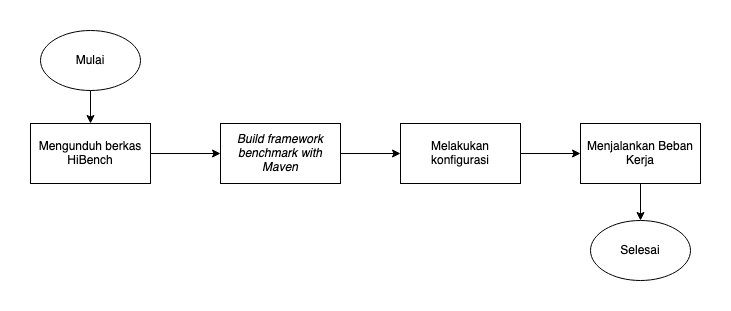
\includegraphics[width=0.9\textwidth]{figures/ch03/hibench-flow.png}
    \caption{Alur Instalasi dan Konfigurasi HiBench}
    \label{fig:hibench-flow}
\end{figure}

\subsection{Eksperimen}
Eksperimen merupakan tahapan yang dilakukan setelah perangkat keras dan perangkat lunak sudah berhasil terpasang. Pada tahapan ini, dilakukan berbagai percobaan untuk menjawab pertanyaan pada masalah yang sebelumnya sudah didefinisikan. Beberapa beban kerja yang akan diuji coba pada tahapan ini dapat dilihat pada Tabel \ref{table:workload}. 

\begin{table}[h!]
\caption{Beban Kerja yang Digunakan}
\label{table:workload}
\resizebox{\textwidth}{!}{%
\begin{tabular}{|l|l|l|l|}
\hline
\multicolumn{1}{|c|}{\begin{tabular}[c]{@{}c@{}}Tipe Beban \\ Kerja\end{tabular}} & \multicolumn{1}{c|}{Nama Beban Kerja} & \multicolumn{1}{c|}{Sumber Data} & \multicolumn{1}{c|}{Perangkat Lunak} \\ \hline
\multirow{3}{*}{\begin{tabular}[c]{@{}l@{}}Micro \\ Benchmarks\end{tabular}} & Sort & RandomTextWriter & \multirow{3}{*}{Hadoop, Spark} \\ \cline{2-3}
 & WordCount & RandomTextWriter &  \\ \cline{2-3}
 & TeraSort & Hadoop TeraGen &  \\ \hline
\end{tabular}%
}
\end{table}

Pengujian dimulai dengan mengeksekusi beban kerja \textit{Micro Benchmarks}, yang terdiri dari \textit{WordCount, Sort, dan TeraSort}, pada DigitalOcean menggunakan parameter data yang divariasikan, yaitu {1GB; 5 GB; 10GB; 25 GB; dan 50 GB}. Parameter input data dapat disesuaikan pada berkas \textit{hibench.conf}. Hasil yang diukur berupa lama waktu eksekusi (\textit{execution time}) dan \textit{throughput per node}. Uji coba yang dijalankan pada HiBench dilakukan sebanyak masing-masing satu uji coba. Pengujian secara lengkap sesuai pada Tabel \ref{table:eksperimen}. Hasil dan konfigurasi dari setiap pengujian dapat diakses melalui berkas \textit{HiBench Report} yang nantinya akan diproses lebih lanjut pada tahap analisis dan evaluasi.

\begin{table}[h!]
\caption{Eksperimen yang Akan diuji Coba}
\label{table:eksperimen}
\resizebox{\textwidth}{!}{%
\begin{tabular}{|l|l|l|c|}
\hline
\multicolumn{1}{|c|}{Beban Kerja} & \multicolumn{1}{c|}{Input Data} & \multicolumn{1}{c|}{\begin{tabular}[c]{@{}c@{}}Perangkat \\ Lunak\end{tabular}} & Hasil yang Diukur \\ \hline
Sort, TeraSort, WordCount & 1 GB & Hadoop & \multirow{10}{*}{\textit{\begin{tabular}[c]{@{}c@{}}Execution time, \\ throughput per node\end{tabular}}} \\ \cline{1-3}
Sort, TeraSort, WordCount & 5 GB & Hadoop &  \\ \cline{1-3}
Sort, TeraSort, WordCount & 10 GB & Hadoop &  \\ \cline{1-3}
Sort, TeraSort, WordCount & 25 GB & Hadoop &  \\ \cline{1-3}
Sort, TeraSort, WordCount & 50 GB & Hadoop &  \\ \cline{1-3}
Sort, TeraSort, WordCount & 1 GB & Spark &  \\ \cline{1-3}
Sort, TeraSort, WordCount & 5 GB & Spark &  \\ \cline{1-3}
Sort, TeraSort, WordCount & 10 GB & Spark &  \\ \cline{1-3}
Sort, TeraSort, WordCount & 25 GB & Spark &  \\ \cline{1-3}
Sort, TeraSort, WordCount & 50 GB & Spark &  \\ \hline
\end{tabular}%
}
\end{table}

\subsection{Proses Analisis dan Evaluasi Hasil Eksperimen}
Analisis pada penelitian ini dilakukan dengan membandingkan hasil setiap eksperimen yang sebelumnya sudah dilakukan. Data yang akan dianalisis didapatkan melalui data eksperimen sebelumnya pada berkas \textit{hibench.report}. Selanjutnya, tahapan ini ditutup dengan evaluasi terhadap hasil dari analisis yang diperoleh.









%    \chapter{Evaluasi dan Pembahasan}

\section{Tujuan Pengujian}
\blindtext

\section{Skenario Pengujian}
\blindtext

\section{Hasil Pengujian}
\blindtext

\section{Pembahasan}
\blindtext
%    \chapter{Penutup}

\section{Kesimpulan}
\blindtext

\section{Saran}
\blindtext
    %----------------------------------------------------------------%

    % Daftar pustaka
    \renewcommand{\bibname}{Daftar Pustaka}
    %\phantomsection
    \addcontentsline{toc}{chapter}{Daftar Pustaka}
    \printbibliography
    
	\appendix
%\addtocontents{toc}{\setcounter{tocdepth}{-1}}
\addcontentsline{toc}{chapter}{Lampiran}
\part*{Lampiran}
\chapter{Instrumen Pengujian}
\chapter{Instalasi dan Konfigurasi Perangkat Lunak Prasyarat}\appcaption{Instalasi dan Konfigurasi Perangkat Lunak Prasyarat}

Pemasangan dan konfigurasi perangkat lunak adalah hal yang krusial. Sebelum dilakukan pemasangan perangkat lunak penyimpanan dan pemrosesan \textit{big data}, tentunya perlu disiapkan perangkat lunak prasyarat. Perangkat lunak prasyarat yang dibutuhkan meliputi Git, Java 8 dan Maven, Python 3.7, serta Scala 2.12. Langkah-langkah pemasangan dan konfigurasi perangkat lunak akan dijelaskan sebagai berikut,

\begin{enumerate}
  \item Pastikan Droplets pada DigitalOcean sudah dibuat. Masuk ke \textit{Virtual Machine} (VM) yang sebelumnya sudah dibuat melalui \textit{Console} yang berada pada laman konfigurasi Droplets DigitalOcean.
	\begin{center}
	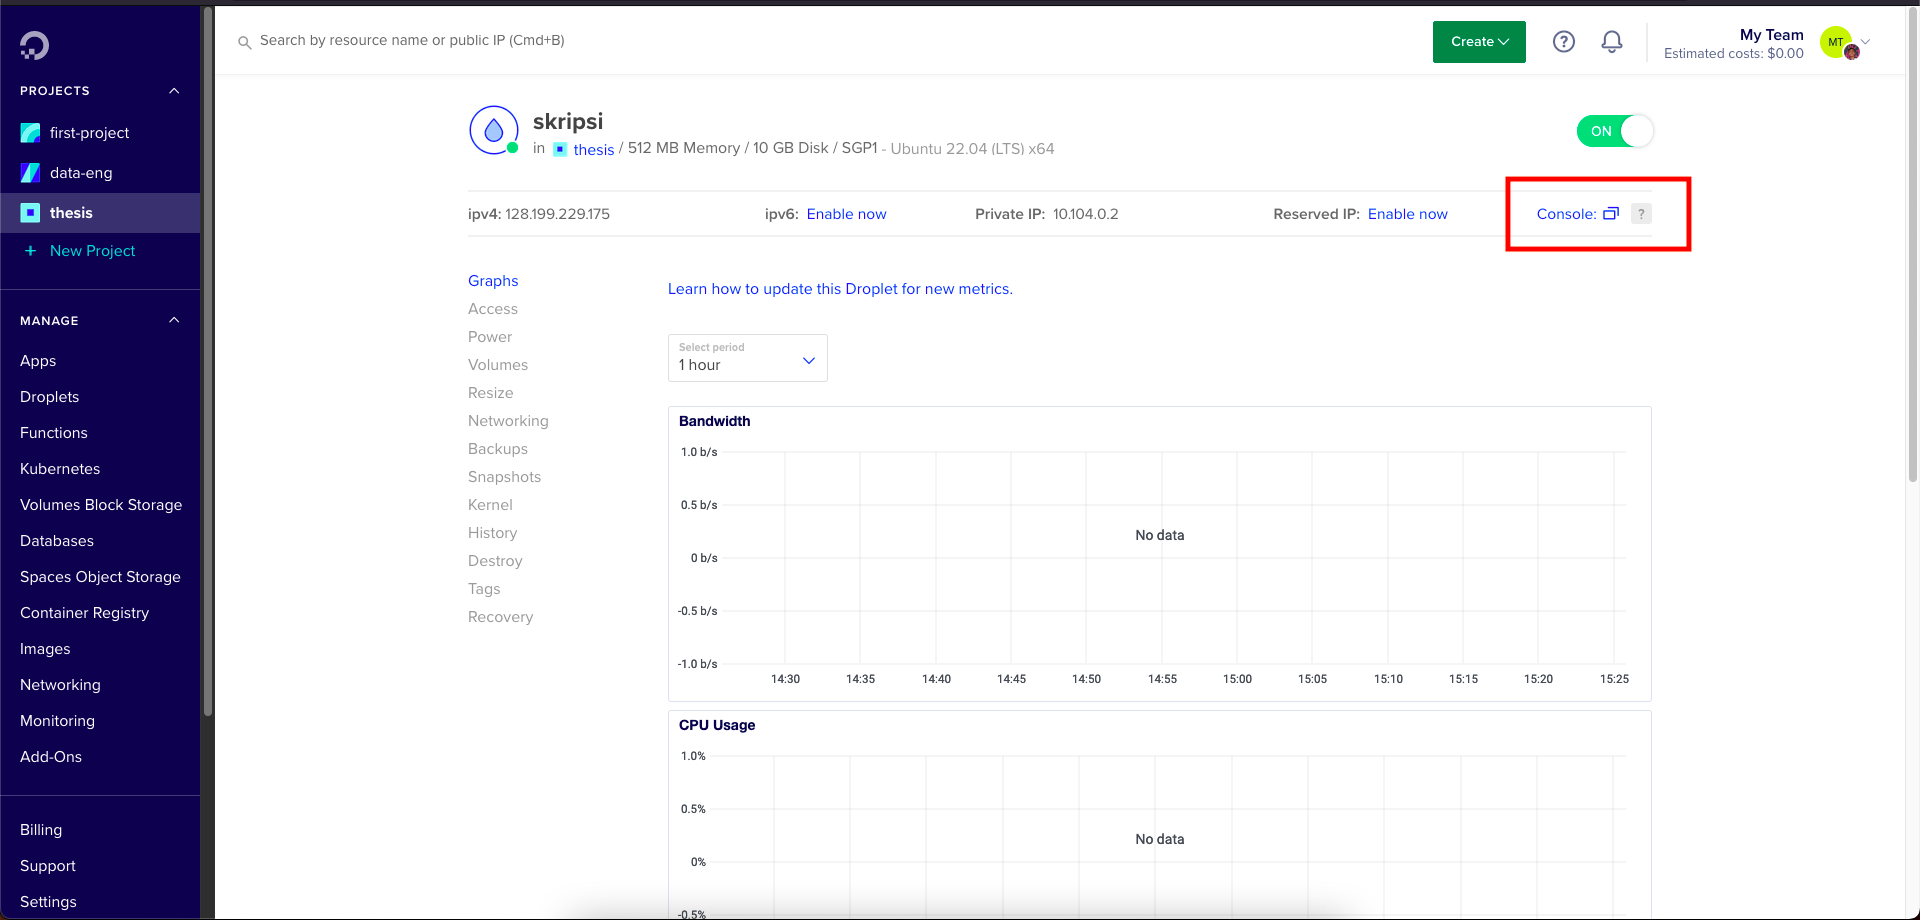
\includegraphics[width=1\linewidth]{figures/ch99/ap1/5.png}
	\end{center} 
  \item Jika Droplets baru saja dibuat, perlu dilakukan pembaruan \textit{index} pada \textit{package management}. \textit{Package management} adalah sistem atau sekumpulan alat yang digunakan untuk mengotomatiskan penginstalan, peningkatan, konfigurasi, dan penggunaan perangkat lunak. Pembaruan \textit{package management} dapat dilakukan dengan \verb|sudo apt update|. 
  \item Membuat Pengguna Baru   \begin{enumerate}
    \item Pertama, buatlah grup baru yang bernama \textit{hadoop} dengan perintah \verb|sudo addgroup hadoop|.
    \item Kemudian, tambahkan pengguna baru \textit{hdfsuser} dalam grup \textit{hadoop} yang sama dengan perintah \verb|sudo adduser --ingroup hadoop hdfsuser|.
    \item Berikan \textit{hdfsuser} izin \textit{root} yang diperlukan untuk pemasangan file. Hak istimewa pengguna \textit{root} dapat diberikan dengan memperbarui file \textit{sudoers}. Buka file \textit{sudoers} dengan menjalankan perintah \verb|sudo visudo|. Tambahkan baris berikut, yaitu \verb|hdfsuser ALL=(ALL:ALL) ALL|.
    \item Sekarang, simpan perubahan dan tutup editor.
    \item Selanjutnya, mari beralih ke pengguna baru yang telah dibuat untuk instalasi lebih lanjut menggunakan perintah \verb|su - hdfsuser|.
  \end{enumerate}
  \item Pengaturan \textit{SSH keys} untuk Hadoop
  \begin{enumerate}
  	\item Hadoop menggunakan \textit{Secure Shell} (SSH) untuk menjalankan proses antara \textit{master nodes} dan \textit{slave nodes}. Penggunaan SSH akan memberikan banyak keuntungan, salah satunya adalah kecepatan. Jika sebuah klaster aktif dan berjalan, komunikasi antar \textit{nodes} akan berjalan terlalu sering. Begitu pula dengan \textit{job tracker} yang harus sering mengirimkan informasi \textit{task to task} dengan cepat.Lakukan pemasangan ssh dan sshd dengan cara \verb|sudo apt-get install ssh| dan \verb|sudo apt-get install sshd| pada terminal.
    \item Selanjutnya, lakukan pembuatan \textit{SSH keys} dengan cara \verb|ssh-keygen -t rsa|. Jika pembuatan \textit{SSH keys} sudah dilakukan, jalankan perintah \verb|cat ~/.ssh/id_rsa.pub >> ~/.ssh/authorized_keys|.
    \item Ubah perizinan berkas dengan perintah \verb|chmod og-wx ~/.ssh/authorized_keys|.
    \item Terakhir, untuk memverifikasi koneksi aman sudah terjadi, lakukan \verb|ssh localhost|.
  \end{enumerate}
  \item Instalasi Git
  \begin{enumerate}
    \item Git dapat dipasang menggunakan perintah \verb|sudo apt install git|. Pengguna akan diminta konfirmasi untuk menginstall. Ketik \verb|y| kemudian tekan enter.
    \item Untuk mengecek versi Git, dapat menggunakan perintah \verb|git --version|.
  \end{enumerate}
  \item Instalasi Python 3.7
  \begin{enumerate}
    \item Python dapat dipasang menggunakan perintah \verb|sudo apt install python3.7|. Pengguna akan diminta konfirmasi untuk menginstall. Ketik \verb|y| kemudian tekan enter.
    \item Untuk mengecek versi Python, dapat menggunakan perintah \verb|python --version|.
  \end{enumerate}
  \item Instalasi Java 8 dan Maven
  \begin{enumerate}
    \item Java 8 dapat dipasang menggunakan perintah \verb|sudo apt install openjdk-8-jre-headless openjdk-8-jdk|. Pengguna akan diminta konfirmasi untuk menginstall. Ketik \verb|y| kemudian tekan enter.
    \item Versi dari Java dapat dilihat menggunakan perintah \verb|java -version|.
    \item Selanjutnya, instalasi Maven dapat dilakukan menggunakan perintah \verb| sudo apt-get -y install maven|.
    \item Informasi dari Maven beserta Java yang digunakan dapat dilihat menggunakan perintah \verb|mvn -version|.
  \end{enumerate}
  \item Instalasi Scala 2.12
  \begin{enumerate}
    \item Scala yang akan dipasang adalah versi 2.12. Jika menggunakan manajer paket, versi yang akan dipasang adalah versi terbaru. Untuk mengunduh versi spesifik dari Scala, dapat menggunakan perintah \verb|sudo apt install wget|, dilanjutkan dengan \verb|sudo wget  https://downloads.lightbend.com/scala/| \verb|2.12.18/scala-2.12.18.deb|.
    \item Scala dapat dipasang menggunakan perintah \verb|sudo dpkg -i scala-2.12.18.deb|.
    \item Versi Scala dapat dilihat melalui perintah \verb|scala -version|.
  \end{enumerate}
\end{enumerate}
\chapter{Instalasi dan Konfigurasi Hadoop}
\label{appendix:C}

Langkah-langkah pemasangan dan konfigurasi Hadoop akan dijelaskan sebagai berikut,

\begin{enumerate}
  \item Unduh Hadoop
  \begin{enumerate}
    \item Pastikan perangkat lunak prasyarat sudah berhasil dipasang dan dilakukan konfigurasi. Sebelum dilakukan pemasangan Hadoop, diperlukan untuk mengunduh berkas Hadoop terlebih dahulu dengan perintah \verb|cd /usr/local|, dilanjutkan dengan \verb|sudo wget https://archive.apache.org/dist/hadoop/|
    \newline \verb|common/hadoop-2.7.7/hadoop-2.7.7.tar.gz|.
    \item Ekstrak berkas Hadoop yang sudah diunduh tadi dengan perintah \verb|sudo tar xvzf hadoop-2.7.7.tar.gz|. Hasil ekstrak berkas Hadoop akan disimpan pada direktori yang sama.
    \item Selanjutnya, untuk memudahkan kedepannya, ganti nama folder Hadoop dengan perintah \verb|sudo mv hadoop-2.7.7 hadoop|.
  \end{enumerate}
  \item Mengubah Kepemilikan Berkas Hadoop
  \begin{enumerate}
    \item Setelah berkas Hadoop sudah berhasil terunduh, selanjutnya ubah kepemilikan berkas Hadoop ke \textit{hdfsuser} yang sebelumnya sudah kita buat dengan perintah \verb|sudo chown -R hdfsuser:hadoop /usr/local/hadoop|.
    \item Tambahkan kekuasaaan untuk membaca, menulis, dan mengeksekusi pada foler Hadoop dengan perintah \verb|sudo chmod -R 777 /usr/local/hadoop|.
  \end{enumerate}
  \item Mematikan \textit{IPv6 Networks}
  \begin{enumerate}
    \item Saat ini Hadoop belum mendukung penggunaan \textit{IPv6 Networks}. Hadoop hanya dibangun dan diuji coba pada \textit{IPv4 Networks}. Untuk mematikan IPv6, dapat dimulai deengan menjalankan perintah \verb|cat /proc/sys/net/ipv6/conf/all/disable_ipv6|.
    \item Jika hasil yang diberikan bukan angka 1, maka beberapa langkah tambahan harus dijalankan. Jalankan perintah \verb|sudo nano /etc/sysctl.conf|, kemudian tambahkan beberapa baris potongan kode berikut pada akhir berkas,
      \begin{lstlisting}[language=bash]
    	# Disable ipv6
		net.ipv6.conf.all.disable_ipv6=1
		net.ipv6.conf.default_ipv6=1
		net.ipv6.conf.lo.disable_ipv6=1
      \end{lstlisting}
    \item Simpan berkas. Kemudian jalankan perintah \verb|sudo sysctl -p| untuk mengaktifkan perubahan.
  \end{enumerate}
  \item Menambahkan Hadoop pada \textit{Environments Variables}
  \begin{enumerate}
    \item Hadoop perlu ditambahkan pada \textit{Environments Variabels} untuk memudahkan dalam melakukan eksekusi. Untuk menambahkannya, jalankan perintah \verb|sudo nano ~/.bashrc|.
    \item Tambahkan beberapa baris kode berikut pada akhir berkas \textit{bashrc}.
      \begin{lstlisting}[language=bash]
		# HADOOP ENVIRONMENT
		export HADOOP_HOME=/usr/local/hadoop
		export HADOOP_CONF_DIR=/usr/local/hadoop/etc/hadoop
		export HADOOP_MAPRED_HOME=/usr/local/hadoop
		export HADOOP_COMMON_HOME=/usr/local/hadoop
		export HADOOP_HDFS_HOME=/usr/local/hadoop
		export YARN_HOME=/usr/local/hadoop
		export PATH=$PATH:/usr/local/hadoop/bin
		export PATH=$PATH:/usr/local/hadoop/sbin
		
		# HADOOP NATIVE PATH
		export HADOOP_COMMON_LIB_NATIVE_DIR=$HADOOP_HOME/lib/native
		export HADOOP_OPTS=-Djava.library.path=$HADOOP_PREFIX/lib
      \end{lstlisting}
    \item Untuk mendapatkan perubahan dapat dilakukan dengan perintah \verb|source ~/.bashrc|.
  \end{enumerate}
  \item Konfigurasi Hadoop
  \begin{enumerate}
    \item Hadoop mengunakan berkas .xml untuk melakukan konfigurasi pada semua prosesnya. Biasanya, letak direktori untuk melakukan konfigurasi terletak pada \verb|$HADOOP_HOME/etc/hadoop|. Oleh karena itu, jalankan perintah \verb|cd /usr/local/hadoop/etc/hadoop/|.
    \item Konfigurasi berkas \textit{hadoop-env.sh} dapat dilakukan dengan perintah \verb|sudo nano hadoop-env.sh|, dilanjutkan dengan menambahkan beberapa baris kode seperti di bawah ini,
       \begin{lstlisting}[language=bash]
		export HADOOP_OPTS=-Djava.net.preferIPv4Stack=true
		export JAVA_HOME=/usr
		export HADOOP_HOME_WARN_SUPPRESS="TRUE"
		export HADOOP_ROOT_LOGGER="WARN,DRFA"
		export HDFS_NAMENODE_USER="hdfsuser"
		export HDFS_DATANODE_USER="hdfsuser"
		export HDFS_SECONDARYNAMENODE_USER="hdfsuser"
		export YARN_RESOURCEMANAGER_USER="hdfsuser"
		export YARN_NODEMANAGER_USER="hdfsuser"
      \end{lstlisting}
    \item Konfigurasi berkas \textit{yarn-site.xml} dapat dilakukan dengan perintah \verb|sudo nano yarn-site.xml|, dilanjutkan dengan menambahkan beberapa baris kode seperti di bawah ini,
       \begin{lstlisting}[language=XML]
		<property>
		<name>yarn.nodemanager.aux-services</name>
		<value>mapreduce_shuffle</value>
		</property>
		<property>
		<name>yarn.nodemanager.aux-services.mapreduce.shuffle.class</name>
		<value>org.apache.hadoop.mapred.ShuffleHandler</value>
		</property>
      \end{lstlisting}
    \item Konfigurasi berkas \textit{hdfs-site.xml} dapat dilakukan dengan perintah \verb|sudo nano hdfs-site.xml|, dilanjutkan dengan menambahkan beberapa baris kode seperti di bawah ini,
       \begin{lstlisting}[language=XML]
		<property>
		<name>dfs.replication</name>
		<value>1</value>
		</property>
		<property>
		<name>dfs.namenode.name.dir</name>
		<value>/usr/local/hadoop/yarn_data/hdfs/namenode</value>
		</property>
		<property>
		<name>dfs.datanode.data.dir</name>
		<value>/usr/local/hadoop/yarn_data/hdfs/datanode</value>
		</property>
		<property>
		<name>dfs.namenode.http-address</name>
		<value>localhost:50070</value>
		</property>
      \end{lstlisting}
    \item Konfigurasi berkas \textit{core-site.xml} dapat dilakukan dengan perintah \verb|sudo nano core-site.xml|, dilanjutkan dengan menambahkan beberapa baris kode seperti di bawah ini,
       \begin{lstlisting}[language=XML]
		<property>
		<name>hadoop.tmp.dir</name>
		<value>/bigdata/hadoop/tmp</value>
		</property>
		<property>
		<name>fs.default.name</name>
		<value>hdfs://localhost:9000</value>
		</property>
      \end{lstlisting}
    \item Konfigurasi berkas \textit{mapred-site.xml} dapat dilakukan dengan perintah \verb|sudo nano mapred-site.xml|, dilanjutkan dengan menambahkan beberapa baris kode seperti di bawah ini,
       \begin{lstlisting}[language=XML]
		<property>
		<name>mapred.framework.name</name>
		<value>yarn</value>
		</property>
		<property>
		<name>mapreduce.jobhistory.address</name>
		<value>localhost:10020</value>
		</property>
      \end{lstlisting}
  \end{enumerate}
  \item Membuat Direktori Hadoop untuk Menyimpan Data
  \begin{enumerate}
    \item Sesuai dengan apa yang ditulis pada \textit{core-site.xml}, langkah pertama yang harus dilakukan adalah membuat direktori sementara untuk dfs menyimpan berkas dengan menjalankan perintah di bawah. Jalankan perintah berikut baris per baris.
       \begin{lstlisting}[language=bash]
		sudo mkdir -p /bigdata/hadoop/tmp
		sudo chown -R hdfsuser:hadoop /bigdata/hadoop/tmp
		sudo chmod -R 777 /bigdata/hadoop/tmp
      \end{lstlisting}
    \item Selanjutnya, jalankan perintah berikut untuk membuat direktori untuk menyimpan berkas data sekaligus mengganti kepemilikan berkas. Jalankan perintah berikut baris per baris.
       \begin{lstlisting}[language=bash]
		sudo mkdir -p /usr/local/hadoop/yarn_data/hdfs/namenode
		sudo mkdir -p /usr/local/hadoop/yarn_data/hdfs/datanode
		sudo chmod -R 777 /usr/local/hadoop/yarn_data/hdfs/namenode
		sudo chmod -R 777 /usr/local/hadoop/yarn_data/hdfs/datanode
		sudo chown -R hdfsuser:hadoop /usr/local/hadoop/yarn_data/hdfs/namenode
		sudo chown -R hdfsuser:hadoop /usr/local/hadoop/yarn_data/hdfs/datanode
      \end{lstlisting}
    \item Konfigurasi untuk Hadoop sudah selesai dan dapat dilanjutkan untuk menjalankan \textit{Resource Manager} dan \textit{Node Manager}
  \end{enumerate}
  \item Menjalankan Hadoop
  \begin{enumerate}
    \item Sebelum menjalankan \textit{Hadoop Core Services}, klaster harus dibersihkan dengan cara melakukan \textit{format} pada \textit{namenode}. Jalankan perintah \verb|hdfs namenode -format|.
    \item Untuk menjalankan layanan Hadoop, dapat dilakukan dengan perintah \verb|start-all.sh|.
    \item Perintah \verb|jps| dapat dilakukan untuk mengecek apakah layanan Hadoop sudah berjalan.
    \item Untuk memberhentikan layanan Hadoop, dapat dilakukan dengan perintah \verb|stop-all.sh| pada terminal.
  \end{enumerate}
\end{enumerate}

\chapter{Instalasi dan Konfigurasi Spark}
\label{appendix:D}

Langkah-langkah pemasangan dan konfigurasi Spark akan dijelaskan sebagai berikut,

\begin{enumerate}
  \item Unduh Berkas Spark
  \begin{enumerate}
    \item Pastikan perangkat lunak prasyarat sudah berhasil dipasang dan dilakukan konfigurasi. Sebelum dilakukan pemasangan Spark, diperlukan untuk mengunduh berkas Spark terlebih dahulu dengan perintah \verb|cd /usr/local|, dilanjutkan dengan \verb|sudo wget https://archive.apache.org/dist/spark/|
    \newline \verb|spark-3.0.3/spark-3.0.3-bin-hadoop2.7.tgz|.
    \item Ekstrak berkas Spark yang sudah diunduh tadi dengan perintah \verb|sudo tar xvf spark-3.0.3-bin-hadoop2.7.tgz|. Hasil ekstrak berkas Spark akan disimpan pada direktori yang sama.
    \item Selanjutnya, untuk memudahkan kedepannya, ganti nama folder Hadoop dengan perintah \verb|sudo mv spark-3.0.3-bin-hadoop2.7 spark|.
  \end{enumerate}
  \item Menambahkan Spark pada \textit{Environments Variables}
  \begin{enumerate}
    \item Spark perlu ditambahkan pada \textit{Environments Variabels} untuk memudahkan dalam melakukan eksekusi. Untuk menambahkannya, jalankan perintah \verb|sudo nano ~/.bashrc|.
    \item Tambahkan beberapa baris kode berikut pada akhir berkas \textit{bashrc}.
      \begin{lstlisting}[language=bash]
		# SPARK ENVIRONMENT
		export PATH=$PATH:/usr/local/spark/bin
		export YARN_CONF_DIR=$HADOOP_HOME/etc/hadoop
		export SPARK_HOME=$PATH:/usr/local/spark/bin
      \end{lstlisting}
    \item Untuk mendapatkan perubahan dapat dilakukan dengan perintah \verb|source ~/.bashrc|.
  \end{enumerate}
  \item Menjalankan \textit{Spark Shell}
  \begin{enumerate}
    \item Pastikan bahwa Spark sudah ditambahkan pada \textit{environmens variables} dengan perintah \verb|spark-submit --version|.
    \item Jalankan layanan Hadoop dengan perintah \verb|start-all.sh|.
    \item Jalankan \textit{spark-shell} dengan YARN menggunakan perintah \verb|spark-shell --master yarn|.
  \end{enumerate}
\end{enumerate}
%\chapter{Instalasi dan Konfigurasi Hive}\appcaption{Instalasi dan Konfigurasi Hive}

Langkah-langkah pemasangan dan konfigurasi Hive akan dijelaskan sebagai berikut,

\begin{enumerate}
  \item Pemasangan Hive
  \begin{enumerate}
    \item Pastikan perangkat lunak prasyarat sudah berhasil dipasang dan dilakukan konfigurasi. Sebelum dilakukan pemasangan Hive, diperlukan untuk mengunduh berkas Hive terlebih dahulu dengan perintah \verb|cd /usr/local|, dilanjutkan dengan \verb|sudo wget https://dlcdn.apache.org/hive/hive-2.3.9/|
    \newline \verb|apache-hive-2.3.9-bin.tar.gz|.
    \item Ekstrak berkas Hive yang sudah diunduh tadi dengan perintah \verb|sudo tar -xzvf apache-hive-2.3.9-bin.tar.gz|. Hasil ekstrak berkas Hive akan disimpan pada direktori yang sama.
    \item Selanjutnya, untuk memudahkan kedepannya, ganti nama folder Hive dengan perintah \verb|sudo mv apache-hive-2.3.9-bin hive|.
  \end{enumerate}
  \item Menambahkan Hive pada \textit{Environments Variables}
  \begin{enumerate}
    \item Hive perlu ditambahkan pada \textit{Environments Variabels} untuk memudahkan dalam melakukan eksekusi. Untuk menambahkannya, jalankan perintah \verb|sudo nano ~/.bashrc|.
    \item Tambahkan beberapa baris kode berikut pada akhir berkas \textit{bashrc}.
      \begin{lstlisting}[language=bash]
		# HIVE ENVIRONMENT
		export PATH=$PATH:/usr/local/hive/bin
      \end{lstlisting}
    \item Untuk mendapatkan perubahan dapat dilakukan dengan perintah \verb|source ~/.bashrc|.
  \end{enumerate}
\end{enumerate}
\chapter{Instalasi HiBench}
%\chapter{Menjalankan Eksperimen Menggunakan HiBench}
\end{document}
